% Chandohasam: mid-submission paper (ACL format).
% Source: paper/draft.md (1 October 2026). Every number is mapped to its file in paper/PROVENANCE.md, and
% every reference is verified (paper/CITATIONS.md). Build with XeLaTeX: `make` in paper/ (see Makefile).
\documentclass[11pt]{article}

\usepackage[preprint]{acl}

% Fonts: XeLaTeX with Times-like text (TeX Gyre Termes) and Noto Sans Telugu for the Telugu examples.
\usepackage{fontspec}
\setmainfont{TeX Gyre Termes}
\setmonofont{Inconsolatazi4-Regular.otf}[BoldFont=Inconsolatazi4-Bold.otf, Scale=MatchLowercase]
\newfontfamily\telugufont{Noto Sans Telugu}[Script=Telugu, Scale=MatchLowercase]
\newcommand{\te}[1]{{\telugufont #1}}

\usepackage{microtype}
\usepackage{amsmath,amssymb}
\usepackage{graphicx}
\usepackage{booktabs}
\usepackage{tabularx}
\usepackage{makecell}
\renewcommand{\theadfont}{\footnotesize}
\usepackage{enumitem}
\usepackage{float}
\usepackage{algorithm}
\usepackage{algpseudocode}

\setlist{nosep, leftmargin=1.1em, labelsep=0.4em}
\newcolumntype{Y}{>{\raggedright\arraybackslash}X}
\renewcommand{\algorithmicrequire}{\textbf{Input:}}
\renewcommand{\algorithmicensure}{\textbf{Output:}}
\algnewcommand{\Symbols}{\item[\textbf{Symbols:}]}
% a statement whose wrapped lines stay indented under its first line
\makeatletter
\algnewcommand{\LongState}[1]{\State\parbox[t]{\dimexpr\linewidth-\ALG@thistlm-1pt\relax}{#1\strut}}
\makeatother
\algrenewcommand\algorithmicindent{1em}
\algrenewcommand\alglinenumber[1]{\scriptsize #1:}
\newcommand{\U}{\textsc{u}}
\newcommand{\I}{\textsc{i}}
% experiment tags: \exref{15}, \exref{3,7} or \exref{22-25,29} in the text link to the results of each
% experiment; \exat{...} marks where those results are reported (an anchor, and the tag as plain text)
\makeatletter
\DeclareRobustCommand{\exref}[1]{{\scriptsize[\def\ex@sep{}\@for\ex@i:=#1\do{\ex@sep
  \expandafter\ex@item\expandafter{\ex@i}\def\ex@sep{, }}]}}
\newcommand{\ex@item}[1]{\in@{-}{#1}\ifin@\ex@range#1\@nil\else\ex@link{#1}\fi}
\def\ex@range#1-#2\@nil{\ex@link{#1}--\ex@link{#2}}
\newcommand{\ex@link}[1]{\hyperref[exp:E#1]{E#1}}
\DeclareRobustCommand{\exat}[1]{{\scriptsize[\def\ex@sep{}\@for\ex@i:=#1\do{\ex@sep
  \expandafter\ex@here\expandafter{\ex@i}\def\ex@sep{, }}]}}
\newcommand{\ex@here}[1]{\in@{-}{#1}\ifin@\ex@hererange#1\@nil\else\ex@anchor{#1}E#1\fi}
\def\ex@hererange#1-#2\@nil{\@tempcnta=#1\relax
  \loop\edef\ex@do{\noexpand\ex@anchor{\the\@tempcnta}}\ex@do
  \ifnum\@tempcnta<#2\relax\advance\@tempcnta\@ne\repeat E#1--E#2}
\newcommand{\ex@anchor}[1]{\phantomsection\label{exp:E#1}}
\newcommand{\exrow}[1]{\ex@anchor{#1}E#1}
\makeatother
\hyphenpenalty=10000
\exhyphenpenalty=10000
\emergencystretch=2em

\title{Chandohasam: Telugu Metrical Poetry Generation with an Exact Metrical Controller and Text Diffusion}

\author{
 \textbf{Samvaran Kashyap Rallabandi},
 \textbf{Mahesh Emani},
 \textbf{Radhe Shyam Salopanthula}
\\
 IIIT Hyderabad
\\
 \small{\{samvaran.rallabandi, mahesh.emani, radheshyam.s\}@research.iiit.ac.in}
}

\begin{document}
\maketitle

\begin{abstract}
A Telugu metrical poem (\textit{padyam}) must satisfy hard constraints on syllable weight (\textit{gaṇa}),
caesura (\textit{yati}) and line-initial rhyme (\textit{prāsa}) while conveying a meaning. We treat padyam
generation as constrained generation: validity can be decided exactly; meaning and quality cannot. We
report four results. (1)~A rules-as-data controller for 37 metres: a minimal labelled automaton (DAWG) of
1,431 states that accepts exactly the 370,315 legal lines, with yati and prāsa engines; it identifies 7,355
of 7,365 labelled poems of Pothana's \textit{Bhāgavatamu} and none as a wrong metre. (2)~Diagnostics: free
generation from three open models gives 0 of 1,665 poems in metre, and a 262K subword vocabulary covers only
10.6\% of the syllable types of Telugu verse. (3)~Three constrained decoding strategies that put the controller inside
autoregressive, block-diffusion and masked-diffusion generators: all 5,550 constrained poems are in metre, but the share of real words falls to
10.7--20.8\% for subword models, while our 120M syllable-level diffusion model keeps 36.9\%. (4)~An audited
corpus and a deterministic poetics suite derived from the \textit{Kāvyālaṅkārasaṅgrahamu}. We close with a
plan for fine-tuning and a 500-poem human study.
\end{abstract}

\section{Introduction}\label{sec:intro}

Telugu \textit{padyams} are composed in metres that fix the weight of every syllable (\textit{akṣara}) of
a line, a caesura (\textit{yati}) at which an akṣara must agree in sound with the line's first akṣara, and
a rhyme (\textit{prāsa}) on the second akṣara of every line. Large language models do not satisfy these
constraints. Prompted once per poem, Gemini 3.7 Flash wrote 255
poems, of which 91 (35.7\%) are strictly valid under our engines (Appendix~\ref{app:pilot1}) \exref{1}. Three
open models (Gemma-4 E4B, Gemma-4 26B-A4B and DiffusionGemma 26B-A4B) write 0 of 1,665 poems in metre when
left free (\S\ref{sec:form}) \exref{22}. The difficulty is not that the rules are unknown. They are codified in the
prosody treatises, such as the seventeenth-century \textit{Appakavīyamu} \citep{appakavi1656}, and are
exact.

\paragraph{Problem statement.}
\begin{itemize}
\item \textbf{Poems and scansion.} Let $\Sigma$ be the set of akṣaras. A poem is a sequence of pādas
  $y = (y_1, \dots, y_P)$, $y_p \in \Sigma^*$. Scansion maps an akṣara sequence to a \emph{set} of weight
  strings over $\{\U, \I\}$ (guru, laghu). It is a set because a light akṣara before a conjunct is heavy,
  and some akṣaras have two accepted readings.
\item \textbf{Metres.} A metre $M$ fixes the number of pādas and a slot $s(p)$ for each; a finite language
  $L_s \subseteq \{\U, \I\}^*$ for each slot, given by its gaṇa grammar; yati seats $K_s$, at which the
  akṣara must be in sound-class harmony (\textit{maitri}) with the pāda's first akṣara under a rule set
  $R_Y$; and a prāsa relation $R_P$ on the second akṣara of every pāda.
\item \textbf{Validity.} $y$ is \emph{valid} for $M$, $\mathrm{Valid}_M(y)$, when every pāda has a reading in
  $L_{s(p)}$ and the yati and prāsa relations hold.
\item \textbf{The task.} Given a meaning $m$ (a prose \textit{bhāvam} or a topic) and a metre $M$, generate
  $y$ with $\mathrm{Valid}_M(y)$ that expresses $m$ in fluent, real Telugu and has the qualities the
  tradition values (the \textit{guṇas}).
\end{itemize}
Validity is decidable exactly, because every $L_s$ is finite and therefore regular. Meaning and quality
are not.

\begin{figure}[t]
\centering
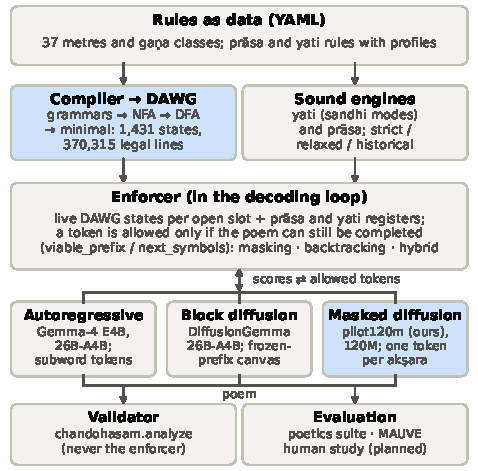
\includegraphics[width=0.92\columnwidth]{figures/fig1_system_overview.pdf}
\caption{System overview. Metre rules (YAML) compile into the DAWG and the yati and prāsa engines. An
enforcer consults them inside the decoding loop of any generator. A separate validator and the evaluation
suite score the finished poem.}
\label{fig:overview}
\end{figure}

\paragraph{Approach} (Figure~\ref{fig:overview}). We separate the decidable part from the rest. A
deterministic controller decides validity exactly and is used \emph{inside} the decoding loop, so every
generated poem is valid by construction; a generator supplies the language and the meaning; and a separate
evaluation suite measures what validity does not. Our generator of choice is a masked diffusion language
model with one token per akṣara: its units are the metre's units, and diffusion lets an akṣara be chosen
with both of its neighbours in view.

\paragraph{Research questions and contributions.}
\textbf{RQ1:} Can validity be decided exactly for the metres of Telugu? We build and validate a rules-as-data
controller for 37 metres (\S\ref{sec:controller}). \textbf{RQ2:} Why do pretrained models fail at it? The
failure lies in their units, not in their exposure to the rules (\S\ref{sec:why}). \textbf{RQ3:} Can
validity be guaranteed across generator architectures, and at what cost? We introduce three constrained
decoding strategies (masking only, masking with backtracking, hybrid), use them in three kinds of generator,
and measure the cost (\S\ref{sec:integration}, \S\ref{sec:form}). \textbf{RQ4:} How
can we measure what validity does not capture? We audit a 15,415-record corpus with a control for every
audit metric (\S\ref{sec:data}) and build a deterministic poetics suite from the
\textit{Kāvyālaṅkārasaṅgrahamu} \citep{ramarajabhushana_kas1920} (\S\ref{sec:eval}). Whether fine-tuning
closes the meaning gap under the constraint is the remaining work (\S\ref{sec:remaining}).

\section{Related Work}

\paragraph{Poetry under form constraints.} Form has been controlled by two routes. The \emph{soft route}
learns or prompts for form and filters failures: Deep-speare models metre jointly with language for English
sonnets \citep{lau2018deepspeare}; SongNet adds format, position and segment symbols \citep{li2020songnet};
PoeLM trains on non-poetic text with codes for length and end rhyme and keeps samples that pass
syllable-count and rhyme filters, as only 31\% (Spanish) and 23\% (Basque) of raw samples meet the
constraints \citep{ormazabal2022poelm}; and a Bangla adaptation adds control tokens for rhyme, mātrā count,
word count and line boundaries, then filters and re-ranks \citep{amina2025}. These controls are aggregate,
and validity comes from filtering, not from the model. The \emph{hard route} constrains decoding: finite-state acceptors for rhythm and rhyme
\citep{ghazvininejad2016}, lexically constrained beam search \citep{hokamp2017,lu2021neurologic},
grammar-constrained decoding \citep{geng2023grammar} and finite-state indexing of the vocabulary
\citep{willard2023outlines}. For Sanskrit, Chandomitra translates English prose into \textit{anuṣṭubh}
verse with 99.86\% metrically valid output under constrained decoding, but human raters score the semantic
coherence of the constrained system at 2.13 out of 5, against 3.78 for an unconstrained instruction-tuned
model \citep{jagadeeshan2026chandomitra}; Pingala reaches near-perfect metrical conformity by biasing
decoding towards complete words at pāda boundaries \citep{jagadeeshan2026pingala}. Meaning under the
constraint is the open problem. PoetryDiffusion pairs continuous diffusion over word embeddings with a
separately trained BERT-based controller for format, rhyme and tone \citep{hu2024poetrydiffusion}. Our
controller is exact instead, and our decoding strategies serve autoregressive and diffusion generators alike.

\paragraph{Computational prosody.} Finite-state scansion exists for English \citep{hulden2013zeuscansion}
and for Ancient Greek hexameter \citep{schumann2021hexameter}. Sanskrit metre identification compares a
line's weight string with known patterns \citep{melnad2015,rajagopalan2018user,terdalkar2023};
Chandojñānam also uses the edit distance to the nearest pattern to suggest corrections \citep{terdalkar2023}.
For Telugu, \citet{boddu2025chandassu} score existing poems against metre patterns and release the
Chandassu dataset, which we audit and use. We differ in compiling every metre into one minimal automaton
\citep{rabin1959,moore1956,daciuk2000,blumer1985}, which both decides validity and answers the prefix
queries a decoder needs.

\paragraph{Discrete diffusion language models.} Continuous diffusion on embeddings was first used for
controllable text \citep{li2022diffusionlm}. Discrete diffusion over tokens was introduced by D3PM
\citep{austin2021d3pm}, and score-entropy discrete diffusion outperformed continuous diffusion language
models at GPT-2 scale \citep{lou2024sedd}. Masked diffusion with a simple weighted cross-entropy is now
competitive \citep{sahoo2024mdlm,shi2024md4}, needs no time input \citep{ou2025radd,zheng2025timeagnostic},
and scales \citep{nie2025llada}. Block diffusion interpolates between autoregressive and diffusion decoding
\citep{arriola2025block}. Remasking samplers let a model revise tokens it has already unmasked
\citep{wang2025remdm}.

\paragraph{Data, units and evaluation.} Pretraining text for Telugu comes from IndicCorp v2 and Sangraha
\citep{doddapaneni2023indiccorp,khan2024indicllmsuite}. Corpus audits show that collected text must be
checked before it is trusted \citep{kreutzer2022quality,dodge2021c4}, and deduplicating training data
reduces memorisation and train--test overlap \citep{lee2022dedup}. Subword vocabularies split Telugu
akṣaras (\S\ref{sec:why}); our model uses one token per akṣara. MAUVE compares distributions of generated
and human text \citep{pillutla2021mauve}; LLM judges rate text quality \citep{zheng2023judge,liu2023geval};
human protocols annotate poetry for aesthetic response \citep{haider2020poemo}. For Sanskrit, computational
work has detected figures of sound (anuprāsa, yamaka) \citep{barbadikar2024anuprasa,barbadikar2023yamaka}
and of meaning (upamā) \citep{jadhav2025upama}, and has analysed a poem through the schools of Sanskrit
poetics \citep{sandhan2025aesthetics}. For English poetry, style has been measured from word frequency and
sound \citep{kao2012style}.

\section{Data and its Audit}\label{sec:data}

\paragraph{Evaluation corpora.} Four files share one record format (Table~\ref{tab:corpora}): Pothana's
\textit{Āndhra Mahābhāgavatamu}, from an online compilation that gives word glosses and meanings
\citep{pothana15c}; Vemana's \textit{śatakam}; Kuchimanchi Timmakavi's pure-Telugu \textit{Rāmāyaṇamu};
and the Chandassu dataset \citep{boddu2025chandassu}, from its Kaggle release \citep{boddu2025kaggle}.
Together they hold 15,415 records, of which 12,704 are verse poems \exref{2}. Outside the Bhāgavatamu, meanings and
word glosses are machine-written (Gemini batch runs), and every English meaning is a machine translation of
the Telugu one.

\paragraph{Audit.} We audited the files at five levels: inventory (level 0), prosodic integrity (1),
meaning-to-verse length ratio (2), embedding similarity (3), and diversity, subword fit and duplicates (4).
An audit metric can measure less than its name says (the similarity gate below is one), so every metric here
carries a \textbf{control} that tests whether the number means what it claims.
\begin{itemize}
\item \textbf{The prosodic rules are hard to satisfy by chance} \exref{4}. Material from unrelated poems of the same
  metre passes 14--18\% of yati seats and 0.0--3.7\% of prāsa stanzas, against 73--93\% and 93--100\% for
  real verse.
\item \textbf{The audit found real faults} \exref{3}, such as backslashes inside words, lost pāda breaks and 142
  Vemana poems mislabelled by a heuristic. Fixing them raised the share of fully valid poems from 72.4\% to
  83.5\% (Vemana) and from 63.8\% to 74.0\% (Chandassu).
\item \textbf{The original similarity gate measures translation consistency, not fidelity} \exref{5}. Telugu--English
  meaning pairs pass LaBSE $\geq$ 0.65 \citep{feng2022labse} at 90--98\%, because one translates the other.
  Poem and Telugu meaning, the pair that bears on fidelity, separate right from wrong pairings (AUC
  0.85--0.94) yet clear 0.65 for only 0.7--5.3\% of poems, and an English-only encoder that cannot read
  Telugu ``passes'' 94--99\% of those pairs. Fixed thresholds are not quality gates here.
\item \textbf{Duplicates} \exref{6}. No poem appears in two files, but refrain lines (\textit{makuṭa}) recur: 77.1\% of
  Vemana poems share a whole pāda with another poem, so splits keep refrain groups together.
\end{itemize}

\begin{table*}[t]
\centering\footnotesize
\begin{tabular}{@{}lrlrrrr@{}}
\toprule
file & \thead[r]{records\\(verse)} & \thead[l]{metre\\label} & \thead[r]{valid, relaxed\\(strict)} & \thead[r]{yati seat:\\real / chance} & \thead[r]{prāsa stanza:\\real / chance} & AUC \\
\midrule
Bhāgavatamu & 10,066 (7,366) & compilation & 91.2\% (88.7\%) & 88.5\% / 17.3\% & 99.8\% / 0.2\% & 0.93 \\
Vemana & 1,164 (1,164) & heuristic / engine & 83.5\% (82.6\%) & 92.5\% / 16.6\% & 95.5\% / 0.0\% & 0.94 \\
Kuchimanchi & 1,653 (1,642) & engine & 90.6\% (88.7\%) & 73.5\% / 14.1\% & 99.9\% / 3.7\% & 0.85 \\
Chandassu & 2,532 (2,532) & dataset & 74.0\% (69.9\%) & 87.4\% / 16.4\% & 98.8\% / 0.1\% & 0.93 \\
\bottomrule
\end{tabular}
\caption{The evaluation corpora and their audit. \textit{Valid}: gaṇa, prāsa and yati all hold under the
relaxed (strict) profile. \textit{Chance}: pass rate of material from unrelated poems of the same metre
(relaxed). \textit{AUC}: LaBSE poem--meaning pairs against shuffled pairs \exat{2-5}.}
\label{tab:corpora}
\end{table*}

\paragraph{Training resources.} Fine-tuning will use Telugu poems crawled from the internet and from blogs,
with their meanings (machine-written where none is given). The pretraining corpus has 4.98B tokens of
Telugu from Sangraha, IndicCorp v2 and Wikipedia, without any document that shares a 20-token window with a
known poem. The Bhāgavatamu is held out of fine-tuning (906 validation and 5,411 test poems).

\section{The Metrical Controller}\label{sec:controller}

\paragraph{Rules as data.} The rules live in YAML files, not in code: 37 metres and their gaṇa classes;
64 prāsa rules and 92 yati rules, each with a status that profiles (strict, relaxed, historical) accept or
reject; and sandhi modes for yati (off, a one-sided hypothesis, vowel-only).

\paragraph{From rules to automaton} (Algorithm~\ref{alg:build}, Appendix). (1)~Each metre is written as
a prosodic grammar: poem $\rightarrow$ lines $\rightarrow$ gaṇa classes $\rightarrow$ gaṇas $\rightarrow$
\U/\I. (2)~The grammar is flattened into one right-linear grammar per (metre, line slot), 40 in all; in
strict form, each is an NFA \citep{hopcroft1979}. (3)~The union of the slot NFAs (1,171 states) is
determinised by subset construction \citep{rabin1959} into a DFA of 1,573 states, whose accepting states
carry their (metre, slot) labels. (4)~Moore partition refinement \citep{moore1956}, started from the
partition by label set, gives the minimal labelled automaton: 1,431 states and 2,514 edges \exref{7}.
The result is a minimal, deterministic, acyclic automaton \citep{daciuk2000}. We call it a DAWG (directed
acyclic word graph), the name \citet{blumer1985} gave to an automaton that recognises the subwords of a
text. It accepts exactly the 370,315 legal lines and builds in under half a second. Minimisation matters:
a trie of these lines would need 1,417,226 states. Figure~\ref{fig:dawg} shows the idea on a toy slot.

\begin{figure*}[t]
\centering
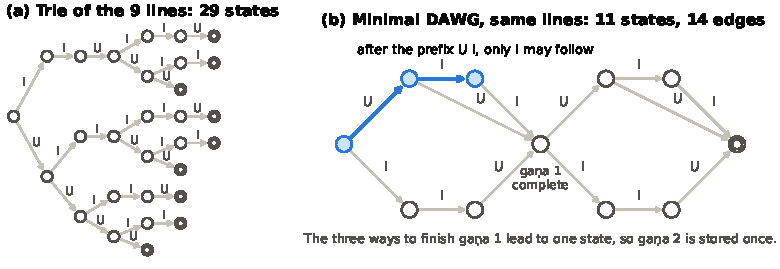
\includegraphics[width=0.8\textwidth]{figures/fig2_dawg_two_panel.pdf}
\caption{The DAWG idea on a toy slot of two gaṇas, each \U\U, \I\I\U\ or \U\I\I: (a) the trie of its 9 legal
lines has 29 states; (b) merging states with equal futures leaves 11 states and 14 edges. After the prefix
\U\,\I, only \I\ may follow: this is the query the decoder asks.}
\label{fig:dawg}
\end{figure*}

\paragraph{Queries.} \texttt{identify} walks a poem's scansion lattice, so open readings (\textit{vikalpa})
are tried together rather than enumerated, and returns every metre and slot that accept and where each
rejected metre dies. \texttt{viable\_prefix} and \texttt{next\_symbols} return the symbols after which some
metre slot can still be completed (co-reachable label sets): the query a decoder asks at every step.
\texttt{segment} returns the gaṇa division and the yati positions that the sound engines check. 16,979 legal lines (4.6\%) fit more than one metre,
16,416 of them shared by \textit{sīsamu} and \textit{taruvōja}; they are reported as ambiguous and never
resolved by guessing.

\paragraph{Validation} (Appendix Table~\ref{tab:controller}). On canonical verse, the DAWG identifies 7,355 of the
7,365 Bhāgavatamu poems that the compilation labels with a catalogue metre (99.86\%) as that metre, none as
a different metre, and 10 as none \exref{8}. Against the per-akṣara weights distributed with the Chandassu dataset
\citep{boddu2025chandassu}, 99.10\% of akṣaras agree \exref{9}. 541 tests pass, including an equivalence check between
every grammar and its automaton by full enumeration, and agreement with a brute-force identification oracle
on valid, mutated and random stanzas \exref{10}. \textbf{Yati} is where the printed text and the rule diverge most.
Pothana's poems pass yati at 63.6\% when no sandhi is assumed, and at 90.7\% when a one-sided sandhi
hypothesis is allowed \exref{11}: sandhi, which the printed text does not show, explains most apparent yati faults.


\section{Integrating the Controller with Generators}\label{sec:integration}

\paragraph{The enforcer} (Figure~\ref{fig:overview}; Algorithm~\ref{alg:step}, Appendix). At each step the
enforcer keeps the live states of the metre's automaton, built as the DAWG is, and two registers for prāsa
and yati. A candidate token is allowed if, after its akṣaras, some slot can still be completed and the
registers still admit a completion; all other tokens are masked. The weight of an akṣara stays pending until
the next onset is known, since a following conjunct makes it heavy. Because liveness is exact, no run can
reach a dead end and every finished poem is valid; evaluation uses the separate analyser, never the
decoder. We introduce three decoding strategies on the enforcer (Algorithm~\ref{alg:decode}):
\emph{masking only}, which samples from the allowed tokens; \emph{masking with backtracking}, which rewinds to
a checkpoint and raises the temperature when the allowed set or its mass collapses; and \emph{hybrid}, which
re-ranks the allowed tokens towards completing the line.

\paragraph{Autoregressive models.} For Gemma-4 E4B and 26B-A4B
\citep{gemma4_2026,hf_gemma4_e4b,hf_gemma4_26b}, the enforcer masks the next-token distribution. A subword
token may span several akṣaras, and all of them are checked. The prompt states the metre's rules, generated
from the catalogue, and a topic.

\paragraph{Block diffusion.} For DiffusionGemma 26B-A4B \citep{hf_diffusiongemma}, which samples block by
block, the constraint acts through a frozen-prefix canvas: tokens committed under the mask stay fixed while
the model redrafts the rest of the block. Two adaptations were needed: an empty thinking-channel prefill,
and forbidding end-of-text inside the canvas.

\paragraph{Our masked-diffusion model.} \texttt{pilot120m} is a 120M-parameter bidirectional transformer
(12 layers, hidden size 768, rotary positions, SwiGLU), trained from scratch as a masked diffusion language
model \citep{sahoo2024mdlm} with no time input \citep{ou2025radd}; masking, unlike uniform corruption,
marks which positions are still undecided, which the constraint needs. It saw 4.98B tokens of Telugu prose
on a single 8 GB laptop GPU in 2 days 19 hours (test NELBO 1.783 nats per token) \exref{12}. Its tokenizer has 45,591
tokens and gives 99.8\% of the akṣara types of our verse their own token \exref{13}, so the constraint acts on single
syllables and the template position equals the token position. Generation fills a 512-token canvas: the
meaning is given unmasked, and the metre's lines are decoded left to right within the line. Prāsa is
checked by the compiled prāsa rules, and yati by an oracle that returns the yati engine's exact verdict in
its left context. An earlier yati table, used out of context, accepted pairs such as \te{త}--\te{య} that no
poem supports and reached 425 of 555 poems in metre; with the oracle and fixes to the sīsa half-break,
couplet metres and prāsa, the decoder reaches 555 of 555 (\S\ref{sec:form}) \exref{23}.

\section{Experiments}\label{sec:experiments}

All results are on the common grid used for every model unless stated: 37 metres $\times$ 3 topics
$\times$ 5 seeds, 555 poems per model and decoding mode. A poem is \emph{in metre} when it is finished and
its canonical gaṇa, strict prāsa and strict yati (no sandhi assumed) all hold.

\subsection{Why pretrained models fail}\label{sec:why}

The diagnostics use \texttt{gemma-4-E2B-it} and 200 Bhāgavatamu poems (25 from each of 8 metres) with their
meanings.\footnote{The Gemma tokenizer does not add \texttt{<bos>}. Without it, the mean surprisal of verse
is 13.45 nats per token, above the uniform bound $\ln|V| = 12.48$; with it, 6.40 \exref{14}. All analyses prepend
\texttt{<bos>}.}

\paragraph{Free generation fails at chance level.} Given the meaning and the metre's rules, the model writes
0 of 200 poems in any metre, although 172 have four lines; 50.8\% of akṣaras within the template's length
have the wrong weight, about what chance gives \exref{15}. In a logistic regression over steps, neither entropy nor
distance from a word junction predicts a violation; only a rare token does.

\paragraph{Weight is looked up, not computed.} A linear probe at each of the 36 layers predicts the current
akṣara's weight. On the 3,938 tokens whose weight depends on the next akṣara, the best layer is the
embedding layer (84.7\%), below a lookup of the current akṣara (88.7\%) and far below one that also sees the
next onset (99.1\%) \exref{16}.

\paragraph{Reading verse shows no sense of the metre.} Verse is harder than its own meaning (6.40 against
5.35 nats; 186 of 200 pairs); pāda starts are \emph{less} surprising than other word starts; and prāsa and
yati seats do not become easier once their anchor is fixed \exref{14}.

\paragraph{Exposure bias is not the main cause.} Under teacher forcing the top choice has the template weight
in 68.4\% of slots (51.0\% when free), so even with the poet's own prefix it misses about a third \exref{15}.
Bidirectional context does not help by itself: DiffusionGemma, which revises within a block, writes 0 of 555
poems in metre when free \exref{22}.

\paragraph{The units do not match.} The 262,144-token Gemma vocabulary has 475 single-akṣara tokens,
covering 10.6\% of the 3,612 akṣara types of our verse (81.9\% of occurrences; ours: 99.8\%) \exref{13}, and
15.5--21.8\% of its token boundaries in verse fall inside an akṣara \exref{17}. A model that emits two or three
syllables at once cannot choose one syllable's weight.

\paragraph{Steering is not an alternative.} Register (verse against prose) is linearly separable from layer
1 (0.978) \exref{18}, and per-metre directions mirror the symbolic distance between metres at 34 of 36 layers (peak
Spearman 0.77) \exref{19}. But no metre-against-metre direction is consistent across poems (all 28 pairs below 0.16
coherence, under a 0.32 threshold) \exref{20}, even on 357 edited contrast poems \exref{21}. Metre is encoded as an average, not
as a direction to steer with, which motivates a hard constraint.

\subsection{Form by construction, and its cost}\label{sec:form}

Table~\ref{tab:grid} gives the main results; Appendix Table~\ref{tab:fullgrid} gives every decoding
strategy \exref{22-25}.
\begin{itemize}
\item \textbf{The constraint guarantees form.} All 4,995 constrained poems of the three Gemma models are in
  metre, and so are the 555 masked poems of \texttt{pilot120m}; free generation gives 0 of 555 for every
  model. Under the chandas distance (\S\ref{sec:eval}), free poems are \emph{farther} from the requested
  metre than prose cut to the metre's line lengths (mean skill $-0.20$ to $-0.33$) \exref{25}: the lines are too short.
\item \textbf{The constraint has a lexical cost for subword models.} Words attested in held-out verse (topic
  words excluded) fall from 33.7--37.2\% to 10.7--20.8\% \exref{24}. The metre overrides the model most often at yati
  positions (52\% of steps for E4B, 66\% for DiffusionGemma) \exref{22}. A quarter to four-fifths of the poems reach a
  level of alliteration that 2.7\% of real poems reach, the 26B models build heavy syllables from rare
  clusters with \te{్ర} and \te{్య}, and 83--99\% of the poems are rated obscure (real verse: 10\%) \exref{25}.
\item \textbf{Syllable-level units preserve vocabulary.} Under the same strict rules, \texttt{pilot120m}
  keeps 36.9\% attested words \exref{23,24}, about the subword models' \emph{unconstrained} level, with about twice as
  many distinct real words as their masking-only runs (757 against 323--375): each token is one akṣara, so
  the mask removes syllables, not multi-syllable subwords, and the model can still finish the words it
  starts. The base model has seen no poetry: 19.7\% of its words are single akṣaras (real verse: 5.6\%),
  and it repeats lines. Its \emph{own} mode (Table~\ref{tab:fullgrid}) reaches 45.6\%
  attested words but only 35 of 555 poems under the strict rules (313 under the relaxed profile).
\item \textbf{A rule the decoders read differently.} \texttt{meter\_engine} reads any pāda-final laghu as guru.
  Under the treatise's narrower reading (only before a conjunct), the Gemma poems need no edits, but 376 of
  the 555 masked \texttt{pilot120m} poems have edits at pāda ends (1,147 in all) \exref{25}, and none under the
  engine's reading. The pilot's decoder relies on the lenient rule; the narrower one is an open choice
  (\S\ref{sec:remaining}).
\end{itemize}

\begin{table*}[t]
\centering\footnotesize
\begin{tabular}{@{}llrrrrrrr@{}}
\toprule
model & mode & \thead[r]{in\\metre} & attested & distinct & \thead[r]{single\\akṣara} & \thead[r]{strong\\anuprāsa} & obscure & MAUVE \\
\midrule
Gemma-4 E4B & free & 0 & 33.7\% & 490 & 0.4\% & 0.4\% & 2.2\% & 0.006 \\
 & constrained & 555 & 10.7\% & 323 & 9.2\% & 33.7\% & 91.4\% & 0.057 \\
Gemma-4 26B-A4B & free & 0 & 37.2\% & 545 & 2.0\% & 9.9\% & 0.9\% & 0.009 \\
 & constrained & 555 & 16.9\% & 375 & 16.1\% & 48.1\% & 91.0\% & 0.014 \\
DiffusionGemma 26B-A4B & free & 0 & 34.4\% & 485 & 4.4\% & 19.1\% & 30.3\% & 0.006 \\
 & constrained & 555 & 11.5\% & 333 & 28.7\% & 71.9\% & 98.9\% & 0.011 \\
\texttt{pilot120m} (ours) & free & 0 & 17.9\% & 183 & 5.9\% & 26.7\% & 45.9\% & -- \\
 & constrained & 555 & \textbf{36.9\%} & \textbf{757} & 19.7\% & 33.7\% & 62.9\% & -- \\
\midrule
real verse & -- & -- & -- & -- & 5.6\% & 2.7\% & 10.0\% & 0.965 \\
\bottomrule
\end{tabular}
\caption{The constrained-decoding grid (555 poems per row; masking only for the Gemma models; the other
strategies in Table~\ref{tab:fullgrid}). \textit{Attested}: words of two or more akṣaras found in
held-out verse (topic words excluded); \textit{distinct}: distinct attested words; \textit{strong anuprāsa},
\textit{obscure}: extreme bands of the poetics metrics (Table~\ref{tab:metrics}); \textit{MAUVE}: against real
verse of the same metre mix ($n = 120$ a side, 5 seeds; not run for \texttt{pilot120m}) \exat{22-25} \exref{29}.}
\label{tab:grid}
\end{table*}

\subsection{Evaluating what metre does not capture}\label{sec:eval}

\paragraph{A deterministic poetics suite.} Following the \textit{Kāvyālaṅkārasaṅgrahamu}
\citep{ramarajabhushana_kas1920,ramarajabhushana_kas1945} and the Sanskrit sources it draws on, we built
five metrics; Table~\ref{tab:metrics} gives the definition, formula and rubric of each. Each has a frozen
corpus baseline, a written rubric and a spec that traces every choice to a source.

\begin{table*}[t]
\centering\scriptsize
\renewcommand{\arraystretch}{1.05}
\begin{tabularx}{\textwidth}{@{}>{\raggedright\arraybackslash}p{1.45cm}Y>{\raggedright\arraybackslash}p{4.95cm}>{\raggedright\arraybackslash}p{3.45cm}@{}}
\toprule
metric & definition & formula & poem rubric \\
\midrule
\textit{anuprāsa} (alliteration) & the share of consonant pairs in a line that are the same sound, Simpson's index of concentration \citep{simpson1949diversity}, as a z-score under a chance model with exact moments & $A$ same-sound pairs among $M$ consonant pairs in different akṣaras of a line; $E = qM$, $q = \sum_s p_s^2$ over corpus frequencies; $z = (A - E)/\sqrt{V}$, $V$ the exact chance variance & line levels at $z$ = 1.645, 2.326, 3.090 (none, weak, marked, strong); poem score = mean line level \\
\textit{mādhurya} (euphony) & six classes of akṣara, from Mammaṭa's soft and harsh lists \citep{mammata_kavyaprakasa} and the sonority scale \citep{parker2011sonority}, with a run-load term for harsh akṣaras that pile up & $w$: madhura $+1$, sonorant $+1/2$, voiced 0, voiceless and conjunct $-1/2$, paruṣa $-1$; $M = I - P$, $I = (1/N) \sum_t w_t$, $P = (1/N) \sum_{t\ \mathrm{harsh}} R_{t-1}$, $R$ the run load & harsh $< -0.283 \leq$ leaning harsh $< -0.123 \leq$ balanced $< 0.049 \leq$ leaning soft $< 0.156 \leq$ soft \\
\textit{ojas} (density) & the mean of the shares of akṣaras inside a word and opening with a conjunct, the features of Indic readability formulas \citep{sinha2012readability}; no constant depends on a corpus & $O = (W + J)/2$; $W = 100\,(1 - 1/L)$, the percentage of akṣaras that continue a word ($L$ akṣaras per word); $J$, the percentage that open with a conjunct & light $< 39.3$ (the treatise's example of words apart, 4.61) $\leq \dots < 47.5$ (its ojas example, 4.70) $\leq$ dense \\
\textit{prasāda} (clarity) & surprisal under an interpolated akṣara trigram model, the surprisal account of reading effort \citep{hale2001earley,smith2013predictability}, trained on crawled poems disjoint from the evaluation files & $H = -(1/N) \sum_t \log_2 P(a_t \mid a_{t-2}, a_{t-1})$ bits per akṣara; the mass kept for unseen akṣaras grows with the distinct akṣaras seen after a context \citep{witten1991zero} & clear $< 5.12 \leq$ leaning clear $< 5.54 \leq$ ordinary $< 6.33 \leq$ leaning obscure $< 7.06 \leq$ obscure \\
chandas distance & the exact edit distance from a poem to every line its metre accepts, by dynamic programming over the automaton \citep{wagner1974order,mohri2003edit}, plus yati and prāsa edits from the engines (Algorithm~\ref{alg:chandas}) & $D$ = weight + yati + prāsa edits; $r = D / \max(n, N)$, $n$ and $N$ the akṣaras of the poem and of the nearest valid one; $S = 1 - r / r_{\mathrm{chance}}(m)$, scaled by the metre's chance rate & exact ($D = 0$), slip, partial, weak, unmetered ($r$ at or above the metre's chance cut) \\
\bottomrule
\end{tabularx}
\caption{The poetics suite: the definition, formula and poem rubric of each metric. Each metric's spec,
baseline and validation are in \texttt{poetry\_metrics/} \exref{26}.}
\label{tab:metrics}
\end{table*}

\paragraph{Validation.} The texts' own examples are placed as the texts place them: the treatise's anuprāsa
example sits at the 97th percentile of reference poems; \textit{mādhurya} puts every soft example above
every harsh one (24 of 24 pairs; 23 without the run-load term); \textit{ojas} orders all 8 dense/light pairs
built from the texts' examples (5 are contrasts a text states), and \textit{prasāda} the 5 clear/obscure
pairs; and the chandas distance finds the faults of the commentary's two broken verses in the pādas the
commentator names. Under the engine's reading of a pāda-final laghu, it is zero exactly when
\texttt{meter\_engine} accepts the poem (12,672 of 12,672 labelled poems) \exref{26}.

\paragraph{The admission test.} The proposal admits a metric only if it declines monotonically when verse
is degraded (word shuffle, metre breaking, filler, synonym swap), and requires metrically valid nonsense to
be rejected by every meaning metric. The chandas distance declines under all four and is admitted \exref{27}. Prasāda
declines under three and rises under the synonym swap, which substitutes plainer glosses, as a clarity
metric should; it rejects the nonsense (200 of the 4,995 constrained poems rate ``ordinary'' or clearer \exref{25}) and
is admitted. The sound metrics describe texture: anuprāsa declines under shuffle and swap, mādhurya and ojas
ignore word order, and both sound metrics rise under filler (a line of \te{మ} is ``strongly alliterative''
and ``soft''); they are read only behind the prasāda gate.

\paragraph{MAUVE.} MAUVE \citep{pillutla2021mauve}, computed with the 300M EmbeddingGemma encoder
\citep{embeddinggemma2025}, passed our gate on canonical Pothana (same-poet halves 0.957, structure-matched
gibberish 0.005; Appendix Table~\ref{tab:mauve}) \exref{28}. Against real verse of the same metre mix (120 poems a side,
5 seeds), every generated set is at the floor (0.006--0.057, against 0.965 for real against real and 0.128
for akṣara-shuffled verse) \exref{29}; mean-pooled Gemma-3-1B states \citep{gemma3_2025} agree (0.005--0.014). MAUVE
reads register and vocabulary, not order or metre: word-shuffled verse still scores 0.91, and Pothana's own
prose 0.015. It cannot tell fluent modern Telugu (the free baselines) from metrically valid nonsense, which
\textit{prasāda} separates (5.4--6.7 against 10.6--12.6 bits per akṣara), and the differences between cells
(0.01--0.05) are of the order of the seed-to-seed spread. We keep it only as a floor check. A Gemma-3-1B
perplexity judge fails on verse too: it separates real from word-shuffled prose (16.9 against 64.9), but
rates real verse at 113, shuffled verse at 150, and repetitive output better than both \exref{30}.

\section{Discussion and Limitations}\label{sec:discussion}

\paragraph{What is shown.} Metrical validity in Telugu can be decided exactly and enforced inside the decoding
loop of very different generators; pretrained models fail through their units and their treatment of
weight, not through ignorance of the rules; and with akṣara-level units the hard constraint stops destroying
vocabulary.

\paragraph{Śabda and artha.} A padyam is judged by the balance (\textit{samanvaya}) of śabda and artha,
sound and meaning. Up to this mid-point we have concentrated on the śabda side: the metre (\textit{chandas})
and the sound of the line. The artha side is next, and this is where a word-resolution metric comes in: how
much of a poem resolves into real words. Until such a metric and a coherence metric are in place, the
śabda metrics mean little, because repetitive gibberish of consonants games them (a line of \te{మ} is
``strongly alliterative'' and ``soft'', \S\ref{sec:eval}). We will build both on a macro dictionary and add
lexical gates on the same basis; besides fine-tuning, they are what is meant to bring coherence
(\S\ref{sec:remaining}).

\paragraph{What is not shown yet.} \emph{No model writes good padyams}: our base model has seen no poetry,
and its constrained output is fragmented and repetitive. \emph{The revision hypothesis is untested}:
the ability to revise a choice motivates diffusion, but our sampler fills positions in any order and never
revises one. \emph{Meaning has not been measured by people}: every
automatic metric here measures form, sound or familiarity. \emph{The tools have limits}: the yati engine is
the weakest on canonical text, because sandhi is unwritten; five-pāda forms are not accepted; and
engine-assigned labels (Vemana, Kuchimanchi) cannot validate the engine.

\section{Remaining Work and Timeline}\label{sec:remaining}

The next phase, to the end of the project on 1 November 2026, adapts the diffusion architecture to poetry,
fine-tunes the models exhaustively, and measures meaning with people. Every stage has a gate; if one is
missed, the study proceeds with the last model that passed. G1: poem NELBO below the base model's, general
NELBO up by under 2\%; G2: the meaning lowers the poem's NELBO; G3 (200 validation meanings): metre $\geq$
99\%, prāsa and yati within 5 points of real poems, $\leq$ 3\% non-words; G4: the meaning score rises within
the copy and diversity guards.
\begin{enumerate}
\item \textbf{2--7 Oct, mid submission:} the human-study interface, rubric and rater recruitment; the test
  split frozen.
\item \textbf{5--14 Oct, architectural adaptation} (G1, G2; G3): continued pretraining on poem + meaning
  documents ($\approx$4 h); multi-task fine-tuning (meaning $\rightarrow$ poem, with explainer, gloss and
  infill tasks) on a canvas with the meaning, a metre header and a register tag ($\approx$13--15 h with a
  learning-rate sweep); a revision test against a remasking sampler \citep{wang2025remdm} with
  validator-triggered remasking; and the rule choices (yati strictness, the pāda-final laghu) on
  validation data.
\item \textbf{5--18 Oct, word resolution and coherence (artha):} both metrics built on a macro dictionary
  and admitted by the suite's test before the automatic evaluation, and lexical gates on the same
  dictionary.
\item \textbf{12--21 Oct, exhaustive fine-tuning} (G4): ablations; rejection-sampling self-training with
  the engines as verifiers ($\approx$5--6 h a round); baselines: retrieval (valid by construction), a local
  few-shot LLM with engine filtering, a matched-size autoregressive model (to isolate diffusion), and the
  constrained Gemma grids; the 523M scale-up if G3 passes; the model table on the test split.
\item \textbf{19--24 Oct, automatic evaluation} of every system on the held-out Bhāgavatamu test split,
  each measure against the real-poem ceiling and the shuffled floor: the final automatic results.
\item \textbf{20--29 Oct, human evaluation} of 500 poems stratified by metre and system on an eight-item
  rubric (Appendix~\ref{app:rubric}), with at least two raters per poem and three on a 100-poem overlap:
  the ratings, their agreement, and the metric--item correlations that complete the admission rule.
\item \textbf{26 Oct--1 Nov, final report:} the final paper (1 November) and the release of the
  controller, corpora, suite and ratings.
\end{enumerate}

\begingroup
\exhyphenpenalty=50 % let long model names in the references break at their own hyphens
\bibliography{references}
\endgroup

\clearpage
\appendix
\raggedbottom

\section{Algorithms}\label{app:algorithms}

\begin{table*}[!t]
\centering\scriptsize
\begin{tabularx}{\textwidth}{@{}>{\raggedright\arraybackslash}p{4.1cm}Y@{}}
\toprule
check & result \\
\midrule
automaton and tests \exat{7,10} & 37 metres, 40 slots; 1,431 states, 2,514 edges; 370,315 legal lines; acyclic, minimal; 541 tests pass, including grammar $\leftrightarrow$ automaton equivalence and a brute-force identification oracle \\
identification, Bhāgavatamu (7,365 labelled) \exat{8} & 7,355 as labelled (99.86\%); 0 as a wrong metre; 10 none \\
prāsa, Bhāgavatamu (4,545 poems) \exref{3} & 96.7\% strict, 99.8\% relaxed \\
yati, Bhāgavatamu (7,355), by sandhi policy \exat{11} & strict, none 63.6\%; strict, hypothesis 90.7\%; relaxed, hypothesis 91.4\%; relaxed, vowel-only 99.8\% \\
Chandassu annotation (4,651 poems) \exat{9} & segmentation identical for 74.3\% (1,036 of the 1,196 differences begin at a word-final dead consonant, which the engine attaches to the preceding akṣara and the annotation to the next); weights of the 227,357 akṣaras of identically segmented poems: 99.10\% agree with the engine's canonical reading, 99.76\% within its open readings \\
\bottomrule
\end{tabularx}
\caption{The controller and its validation.}
\label{tab:controller}
\end{table*}

\begin{table*}[!t]
\centering\scriptsize
\begin{tabular}{@{}llrrrrrrr@{}}
\toprule
model & mode & \thead[r]{in\\metre} & attested & distinct & \thead[r]{single\\akṣara} & \thead[r]{strong\\anuprāsa} & obscure & MAUVE \\
\midrule
Gemma-4 E4B & backtracking & 555 & 12.2\% & 394 & 9.3\% & 23.1\% & 83.8\% & 0.037 \\
 & hybrid & 555 & 11.7\% & 355 & 7.9\% & 30.3\% & 89.4\% & 0.035 \\
Gemma-4 26B-A4B & backtracking & 555 & 20.8\% & 525 & 12.0\% & 49.0\% & 83.1\% & 0.015 \\
 & hybrid & 555 & 16.7\% & 436 & 14.1\% & 47.7\% & 87.2\% & 0.027 \\
DiffusionGemma 26B-A4B & backtracking & 555 & 11.6\% & 432 & 25.0\% & 46.7\% & 98.9\% & 0.032 \\
 & hybrid & 555 & 12.9\% & 330 & 26.5\% & 78.9\% & 93.7\% & 0.011 \\
\texttt{pilot120m} (ours) & own & 35 (313 relaxed) & 45.6\% & 1,451 & 17.8\% & 20.5\% & 51.7\% & -- \\
\bottomrule
\end{tabular}
\caption{The other decoding strategies on the grid (555 poems each); free and masking-only runs are in
Table~\ref{tab:grid}, whose columns these are. \textit{Own}: the pilot's own mode (soft yati penalty, 16
particles, soft lexicon), counted under the strict rules \exref{22-25,29}.}
\label{tab:fullgrid}
\end{table*}



\paragraph{Terms used in the algorithms.} An \emph{akṣara} is a syllable; it is \emph{guru} (heavy, \U) or
\emph{laghu} (light, \I). A \emph{gaṇa} is a fixed group of weights, such as bha = \U\I\I. A poem has
\emph{pādas} (lines), and a \emph{slot} is a kind of line that a metre allows: kandamu's odd and even lines are
two slots. At a \emph{yati} seat, the akṣara must agree in sound (\emph{maitri}) with the first akṣara of the
line, the \emph{vaḷi}. By \emph{prāsa}, the second akṣara of every line repeats the consonant of the second
akṣara of line 1. An \emph{automaton} is a graph of \emph{states} joined by edges marked \U\ or \I; a line is
legal when its weights lead from the start state to a \emph{final} state. A \emph{token} is the unit a
language model emits: one akṣara for our model, a subword of one or more akṣaras for the Gemma models.

\begin{algorithm}[H]
\caption{Build the labelled metrical DAWG}\label{alg:build}
\scriptsize
\begin{algorithmic}[1]
\Require the metre catalogue and the gaṇa classes (YAML files)
\Ensure the DAWG $D$ (1,431 states, 2,514 edges; acyclic, as every line has a bounded length), and the
label set $C(q)$ of each state $q$
\Symbols $m$, $s$: a metre and one of its line slots (a vṛtta has one slot; kandamu has
two, its odd and even lines). \U, \I: guru, laghu. $N_{m,s}$: the automaton of the slot, whose
\emph{label} is $(m, s)$. $C(q)$: the labels whose lines can still be completed from state $q$.
\For{each metre $m$ and each slot $s$ of $m$}
  \LongState{write the slot's grammar: one position per gaṇa, each allowing the gaṇas of its class}
  \LongState{split every rule into rules that read one weight (\U\ or \I) each}
  \LongState{turn the grammar into an automaton $N_{m,s}$, and label its final state $(m, s)$}
\EndFor
\LongState{join all the $N_{m,s}$ into one automaton and make it deterministic (subset construction); a
merged state keeps every label of the states it merges}
\State remove the states that cannot reach a final state
\State put the states with the same labels into one group
\Repeat
  \LongState{split a group whose states go to different groups on \U\ or on \I\ (Moore)}
\Until{no group splits}
\State merge each group into one state; the result is $D$
\LongState{for each state $q$, from the ends of the lines back to the start: $C(q) \gets$ the labels of $q$
together with $C$ of each state that $q$ leads to}
\State \Return $D$ and $C$
\end{algorithmic}
\end{algorithm}

\begin{algorithm}[H]
\caption{The enforcer}\label{alg:step}
\scriptsize
\begin{algorithmic}[1]
\Require the metre $M$; the state $\sigma$ of the text so far; the next akṣara $a$ (or a space or a line
break)
\Ensure the new state, or \textsc{dead} if no poem of $M$ can begin with the text
\Symbols The state $\sigma$ has four parts. $Q$: the states of $M$'s automaton (built as in
Algorithm~\ref{alg:build}, for $M$ alone) that the text may be in. $w$: the last akṣaras, whose weight is
still open (a light akṣara before a conjunct is heavy). The \emph{prāsa register}: the consonant of line
1's second akṣara, which the second akṣara of every line must repeat. The \emph{yati register}: the line's
first akṣara (the vaḷi), with which the akṣara at a yati seat must agree in sound (\emph{maitri}).
\State settle the open weights in $w$ by the first consonant of $a$
\State move each state in $Q$ along the settled weights; drop those with no move
\State \textbf{if} $a$ is the second akṣara of a line and breaks the prāsa \textbf{then return} \textsc{dead}
\LongState{drop from $Q$ the states whose gaṇa division puts $a$ on a yati seat where $a$ is not in maitri
with the vaḷi}
\State \textbf{if} no state in $Q$ can still reach the end of the poem \textbf{then return} \textsc{dead}
\State \Return $\sigma$ with $Q$, $w$ and the registers updated
\end{algorithmic}
A token is \emph{allowed} when the state stays alive after all of its akṣaras (cached per state). Liveness
is exact, so decoding never reaches a dead end, and every finished poem is valid. The gaṇa grid acts as a
mask from the first token; yati and prāsa act once their anchor (the vaḷi, line 1's prāsa akṣara) is
written. Meaning has no closed-form check: it is left to the generator and the evaluation.
\end{algorithm}

\begin{algorithm}[H]
\caption{Decoding with three strategies}\label{alg:decode}
\scriptsize
\begin{algorithmic}[1]
\Require a language model; a metre $M$; a strategy (masking only, backtracking or hybrid); a temperature
$\tau_0$
\Ensure a poem $y$ that is valid for $M$
\Symbols $y$: the poem so far; $\sigma$: its enforcer state (Algorithm~\ref{alg:step});
$A$: the allowed tokens; $p$: the model's probabilities for the next token; $\tau$: the temperature
(probabilities are raised to the power $1/\tau$); $c$: the number of backtracks in a row; a
\emph{checkpoint}: a saved copy of $(y, \sigma, \tau)$. The run is \emph{stuck} when fewer than 3 tokens
are allowed, when they hold less than 0.001 of $p$, or after 4 steps without a new akṣara.
\State $y \gets$ the empty poem; $\sigma \gets$ the start state; $\tau \gets \tau_0$; $c \gets 0$
\While{$y$ is not a complete poem}
  \LongState{\textbf{if} the line is complete and cannot grow \textbf{then} add a line break, and go to the
  next step}
  \State backtracking: every third step, save a checkpoint (keep the last 15)
  \State $A \gets$ the allowed tokens; \ $p \gets$ the model's probabilities
  \If{backtracking and the run is stuck}
    \LongState{$c \gets c + 1$; go back $c$ checkpoints; raise $\tau$ by $0.15c$, to at most 1.2; go to
    the next step}
  \EndIf
  \State mask: set $p$ to 0 outside $A$, apply $\tau$, and renormalise
  \If{hybrid}
    \LongState{go down the allowed tokens by probability (at most 100), collecting those that complete the
    line; stop at 3, or at the 10th token if none was found; sample among the collected tokens, or else
    among those 10}
  \Else
    \LongState{sample from the most probable tokens that together hold 90\% of $p$ (top-$p$)}
  \EndIf
  \State add the token to $y$; update $\sigma$; $c \gets 0$
\EndWhile
\State \Return $y$
\end{algorithmic}
After a backtrack, $\tau$ returns to $\tau_0$ over 6 steps; the autoregressive runs use $\tau_0 = 0.7$.
\textit{Block diffusion} commits the model's own proposals left to right while each is allowed and
confident; otherwise the strategy chooses the token at the first open position, and a backtrack returns
committed tokens to noise.
\end{algorithm}

\begin{algorithm}[H]
\caption{Chandas distance}\label{alg:chandas}
\scriptsize
\begin{algorithmic}[1]
\Require the printed lines of a poem, each akṣara with the weights it may take; a metre $m$
\Ensure the distance $D$, and the skill $S$ (1 for a poem in metre, 0 for one no nearer to $m$ than prose)
\Symbols $x$: a printed line, and $x_i$ its $i$-th akṣara; $q$: a state of the slot's own
automaton (built as in Algorithm~\ref{alg:build}); $\mathit{cost}[i][q]$: the fewest edits that read
$x_1 \dots x_i$ and end in state $q$; $n$, $N$: the number of akṣaras in the poem and in the nearest valid
poem; $r$: the edit rate; $r_{\mathrm{chance}}(m)$: the mean rate of prose cut to the line lengths of $m$.
\For{each printed line $x$ and each slot $s$ of $m$}
  \LongState{fill $\mathit{cost}[i][q]$ for $i = 0, 1, \dots$: reading $x_i$ along an edge costs 0 if the
  edge's weight is one that $x_i$ may take, else 1 (substitution); skipping $x_i$ costs 1 (deletion);
  following an edge without reading costs 1 (insertion)}
  \LongState{the line's distance is the lowest cost at a final state after the last akṣara (a pāda-final
  laghu may also read as \U); its path gives the nearest legal line}
\EndFor
\LongState{weight edits: match the lines to the metre's pādas with the fewest edits; a line left over costs
its length, a pāda left empty its shortest line}
\LongState{yati edits: one for each yati seat whose akṣara is not in maitri with the vaḷi}
\LongState{prāsa edits: the fewest pādas to change so that all the pādas rhyme}
\LongState{$D \gets$ the sum of the three, counting once an akṣara that a weight edit already rewrites}
\State $r \gets D / \max(n, N)$; \ $S \gets 1 - r / r_{\mathrm{chance}}(m)$
\State \Return $D$ and $S$
\end{algorithmic}
\end{algorithm}

\section{Additional Tables}\label{app:tables}

\paragraph{Pilot 1}\label{app:pilot1} (one-shot poems from Gemini 3.7 Flash, scored by our engines; strict profile,
compound readings excluded): 91 of 255 (35.7\%) are valid. Valid / poems by metre: utpalamāla 28 / 53,
campakamāla 17 / 52, śārdūla 4 / 46, mattēbha 4 / 40, āṭaveladi 10 / 13, tēṭagīti 9 / 13, sīsamu 0 / 13,
kandamu 8 / 13, utsāhamu 11 / 12 \exat{1}.

\begin{table}[H]
\centering\scriptsize
\begin{tabularx}{\columnwidth}{@{}Yr@{}}
\toprule
condition & MAUVE \\
\midrule
held-out Pothana vs Pothana (1,601) & 0.957 $\pm$ 0.003 \\
line order shuffled (1,601) & 0.906 $\pm$ 0.007 \\
word order shuffled (1,601) & 0.716 $\pm$ 0.034 \\
vṛtta vs jāti, both Pothana (721) & 0.214 $\pm$ 0.029 \\
akṣaras shuffled (1,601) & 0.028 $\pm$ 0.002 \\
Pothana vs Vemana, āṭaveladi only (313) & 0.051 $\pm$ 0.007 \\
structure-matched gibberish (1,601) & 0.005 $\pm$ 0.000 \\
\midrule
real vs real (120) & 0.965 $\pm$ 0.006 \\
real vs its words shuffled (120) & 0.912 $\pm$ 0.065 \\
real vs its akṣaras shuffled (120) & 0.128 $\pm$ 0.042 \\
real verse vs Pothana's prose (120) & 0.015 $\pm$ 0.004 \\
generated poems, 12 model $\times$ decoding cells (120) & 0.006--0.057 \\
the same 12 cells, Gemma-3-1B mean-pooled featurizer (120) & 0.005--0.014 \\
\bottomrule
\end{tabularx}
\caption{MAUVE with \texttt{embeddinggemma-300m}. Top: the gate on Pothana (5 seeds; $n$ per side). Bottom:
controls of the generated-poem comparison (real verse with the matched metre mix, $n = 120$, 5 seeds); for
the Gemma-3-1B featurizer, real against real scores 0.940. The generated cells are in
Table~\ref{tab:fullgrid} \exat{28,29}.}
\label{tab:mauve}
\end{table}

\paragraph{The human-evaluation rubric}\label{app:rubric} (planned; \S\ref{sec:remaining}). (1)~How easy is it to
read? (1--5) (2)~How easy is it to understand immediately after reading? (1--5) (3)~How many words of the
poem are understood? (1--5) (4)~Is the chandassu correct? (0/1) (5)~Is the prāsa correct? (0/1) (6)~Is the
yati correct? (0/1) (7)~Does the poem express the given meaning? (1--5) (8)~How good is it as a poem?
(1--5). Items 1--6 come from the proposal; items 7--8 are added for the study. Three 500-poem pools of
engine-verified real and generated poems are ready for it.

\onecolumn
\section{Metres, Prāsa Rules and Yati Rules}\label{app:rules}

The tables are generated from the engine's rule files by \texttt{paper/scripts/make\_rule\_tables.py}.
\captionsetup{font=scriptsize,skip=3pt}

{\centering\tiny\renewcommand{\arraystretch}{0.92}
\setlength{\tabcolsep}{3pt}
\begin{minipage}[t]{0.47\textwidth}
\centering
\begin{tabularx}{\linewidth}[t]{@{}rlYll@{}}
\toprule
\# & vṛtta (4 pādas) & gaṇas (akṣaras) & yati akṣara & prāsa \\
\midrule
1 & utpalamāla & bha ra na bha bha ra va (20) & 10 & yes \\
2 & campakamāla & na ja bha ja ja ja ra (21) & 11 & yes \\
3 & mattēbhavikrīḍitamu & sa bha ra na ma ya va (20) & 14 & yes \\
4 & śārdūlavikrīḍitamu & ma sa ja sa ta ta ga (19) & 13 & yes \\
5 & sragdhara & ma ra bha na ya ya ya (21) & 8, 15 & yes \\
6 & mahāsragdhara & sa ta ta na sa ra ra ga (22) & 9, 16 & yes \\
7 & tōṭakamu & sa sa sa sa (12) & 9 & yes \\
8 & bhujaṅgaprayātamu & ya ya ya ya (12) & 8 & yes \\
9 & mattakōkilamu & ra sa ja ja bha ra (18) & 11 & yes \\
10 & pañcacāmaramu & ja ra ja ra ja ga (16) & 10 & yes \\
11 & vasantatilakamu & ta bha ja ja gaga (14) & 8 & yes \\
12 & indravajra & ta ta ja gaga (11) & 8 & yes \\
13 & upēndravajra & ja ta ja gaga (11) & 8 & yes \\
14 & śālini & ma ta ta gaga (11) & 7 & yes \\
15 & rathōddhata & ra na ra va (11) & 7 & yes \\
16 & sragviṇi & ra ra ra ra (12) & 7 & yes \\
17 & vidyunmāla & ma ma gaga (8) & 5 & yes \\
18 & lalita & ta bha ja ra (12) & 9 & yes \\
30 & taraḷamu & na bha ra sa ja ja ga (19) & 12 & yes \\
31 & mālini & na na ma ya ya (15) & 9 & yes \\
32 & mānini & bha bha bha bha bha bha bha ga (22) & 7, 13, 19 & yes \\
33 & kavirājavirājitamu & na ja ja ja ja ja ja va (23) & 8, 14, 20 & yes \\
34 & vanamayūramu & bha ja sa na gaga (14) & 9 & yes \\
35 & maṅgaḷamahāśrī & bha ja sa na bha ja sa na gaga (26) & 9, 17 & yes \\
36 & layagrāhi & bha ja sa na bha ja sa na bha ya (30) & 9, 17, 25 & yes; PY \\
37 & layavibhāti & na sa na na sa na na sa na na sa ga (34) & 10, 19, 28 & yes; PY \\
\bottomrule
\end{tabularx}
\end{minipage}\hfill
\begin{minipage}[t]{0.51\textwidth}
\centering
\begin{tabularx}{\linewidth}[t]{@{}rlcYll@{}}
\toprule
\# & metre & pādas & gaṇas of a pāda (lines) & yati & prāsa \\
\midrule
\multicolumn{6}{@{}l}{\textit{jāti}} \\
19 & kandamu & 4 & odd pādas 3, even 5 kanda gaṇas (bha, ja, sa, nala, gaga); no ja in an odd place; 6th gaṇa ja or nala; even pādas end in a guru (80 / 320 lines) & gaṇa 4 (even) & yes \\
20 & utsāhamu & 4 & 7 sūrya gaṇas + a guru (128 lines) & gaṇa 5 & yes \\
21 & taruvōja & 4 & 3 indra, 1 sūrya, 3 indra, 1 sūrya (186,624 lines) & gaṇas 3, 5, 7 & yes \\
22 & dvipada & 2 & 3 indra, 1 sūrya (432 lines) & gaṇa 3 & yes \\
23 & madhyākkara & 4 & 2 indra, 1 sūrya, 2 indra, 1 sūrya (5,184 lines) & gaṇa 4 & yes \\
24 & madhuragati ragaḍa & 2 & 4 four-mātrā gaṇas (625 lines) & gaṇa 3 & yes; PY \\
25 & turagagati ragaḍa & 4 & 8 three-mātrā gaṇas (6,561 lines) & gaṇa 5 & yes; PY \\
26 & hayapracāra ragaḍa & 2 & 4 three-mātrā gaṇas (81 lines) & gaṇa 3 & yes; PY \\
\midrule
\multicolumn{6}{@{}l}{\textit{upajāti}} \\
27 & sīsamu & 4 & 6 indra, 2 sūrya (or the all-laghu form); then an āṭaveladi or a tēṭagīti (186,624 + 1 lines) & gaṇas 3, 7 & no; PY \\
28 & āṭaveladi & 4 & odd pādas 3 sūrya + 2 indra; even pādas 5 sūrya (288 / 32 lines) & gaṇa 4 & no; PY \\
29 & tēṭagīti & 4 & 1 sūrya, 2 indra, 2 sūrya (288 lines) & gaṇa 4 & no; PY \\
\bottomrule
\end{tabularx}
\end{minipage}
\captionof{table}{The 37 metres of the catalogue (\texttt{meter\_rules.yaml}). Vṛtta gaṇas: bha \U\I\I, ja \I\U\I, sa \I\I\U, na \I\I\I, ya \I\U\U, ra \U\I\U, ta \U\U\I, ma \U\U\U, ga \U, va \I\U, gaga \U\U. Sūrya gaṇas: na, ha (\U\I); indra gaṇas: bha, ra, ta, nala, naga, sala. \textit{Yati}: the seat that must agree with the first akṣara (of the pāda, or of gaṇa 1); PY: prāsa-yati, a prāsa match at the seat, is accepted in place of yati. \textit{Lines}: the legal weight strings of a pāda (odd / even pādas; + 1 for the all-laghu sīsamu); a vṛtta has one. Bhāgavatamu poems by label (level-0 inventory): kandamu 2,608, tēṭagīti 1,051, sīsamu 1,048, āṭaveladi 716, mattēbhavikrīḍitamu 586, campakamāla 490, utpalamāla 471, śārdūlavikrīḍitamu 289, mattakōkilamu 41, taraḷamu 23, mālini 12, and 30 in 15 other metres.}
\label{tab:metres}\par}
\medskip

{\centering\tiny\renewcommand{\arraystretch}{0.92}
\begin{tabularx}{\textwidth}{@{}>{\raggedright\arraybackslash}p{2.6cm}Y@{}}
\toprule
family & rules (id: name [status]) \\
\midrule
\textsc{pos} (8) position, scope, normalisation & \textbf{01} Prāsa position (2nd akshara of every pāda) [C]; \textbf{02} Meter eligibility [C]; \textbf{03} Uniformity across meters [I]; \textbf{04} Stanza scope [C]; \textbf{05} Sandhi surface form is what is judged [C]; \textbf{06} Saṃśleṣa [M]; \textbf{07} Druta-sandhi alternative reading [C]; \textbf{08} Dantya \te{ౘ/ౙ} normalisation [C] \\
\textsc{sama} (12) samaprāsa: identity and neutral features & \textbf{01} Samaprāsa [C]; \textbf{02} Vowel neutrality [C]; \textbf{03} \te{ఋ}-tva sahita [C]; \textbf{04} \te{ఌ}-kāra sahita [C]; \textbf{05} Bindu-sahita [C]; \textbf{06} Visarga-sahita [C]; \textbf{07} Drutam following the prāsa akshara is neutral [C]; \textbf{08} Pollu \te{ల్} (or any dead consonant) following the prāsa akshara is neutral [C]; \textbf{09} Dantya and tālavya \te{చ/జ} are savarṇa [C]; \textbf{10} Weight of the prāsa akshara itself is free [I]; \textbf{11} Laghu-yakāra prāsa [Cs]; \textbf{12} Sandhigata prāsa [Cs] \\
\textsc{samyukta} (8) conjuncts & \textbf{01} Conjunct presence must agree (saṃyuktākṣara prāsamu) [M]; \textbf{02} Constituent consonants and their order must be identical (kramamu) [M]; \textbf{03} Dvitvākṣara prāsa [M]; \textbf{04} Three-consonant clusters keep all three in order [M]; \textbf{05} \te{ఋ} inside a conjunct is a vowel [C]; \textbf{06} Pūrṇabindu-pūrvaka saṃyuktākṣara prāsa [Cs]; \textbf{07} Drutam-fused conjunct prāsa (\te{న్}X) [Cs]; \textbf{08} Pollu-\te{ల్}-fused conjunct prāsa (\te{ల్}X) [Cs] \\
\textsc{purvaka} (6) signs before the prāsa akṣara & \textbf{01} Pūrṇabindu prāsa [M]; \textbf{02} Visarga prāsa [M]; \textbf{03} Ardhabindu prāsa [Cs]; \textbf{04A} Khaṇḍākhaṇḍa prāsa within Ananta's restriction (\te{ప/ట}) [Cs]; \textbf{04B} Khaṇḍākhaṇḍa prāsa within Appakavi's restriction (paruṣa after a long vowel) [Cs]; \textbf{04C} Khaṇḍākhaṇḍa prāsa in its wide classical form [R] \\
\textsc{purvakshara} (4) weight of the pre-prāsa akṣara & \textbf{01} Pre-prāsa akshara weight uniformity [M]; \textbf{02} Metrical weight, not vowel length [C]; \textbf{03} Kandamu gana corollary [I]; \textbf{04} Light repha clusters [Cs] \\
\textsc{maitri} (15) accepted or deprecated equivalences & \textbf{SA-SHA} \te{స} $\sim$ \te{శ} sibilant compatibility [R]; \textbf{THA-DHA} \te{థ} $\sim$ \te{ధ} svavargaja prāsa [R]; \textbf{NA-NNA} \te{న} $\sim$ \te{ణ} ubhaya prāsa (1) [R]; \textbf{LA-LLA} \te{ల} $\sim$ \te{ళ} abhēda prāsa [R]; \textbf{RU-RA} \te{ఋ} prāsa [R]; \textbf{RU-HALSAMYUTA} Hal-saṃyuta \te{ఋ} prāsa [R]; \textbf{VIKALPA} Vikalpa prāsa [R]; \textbf{BINDU-SAMSLESHA} Bindu $\sim$ saṃśleṣa spelling of one nasal + stop (\te{ంద} $\sim$ \te{న్ద}) [R]; \textbf{RA-RRA-ORTHO} \te{ర} $\sim$ \te{ఱ} orthographic relaxation (rēpha $\sim$ śakaṭarēpha) [O]; \textbf{SA-SSA} \te{స} $\sim$ \te{ష} ubhaya prāsa (2) [D]; \textbf{LA-DA} \te{ల/ళ} $\sim$ \te{డ} [D]; \textbf{DA-DHA} \te{ద} $\sim$ \te{ధ} [D]; \textbf{SAMYUKTASAMYUKTA} Saṃyuktāsaṃyukta prāsa [D]; \textbf{ANUNASIKA} Anunāsika prāsa [D]; \textbf{MBA-MMA} \te{ంబ} $\sim$ \te{మ్మ} prāsamaitri prāsa (deprecated) [D] \\
\textsc{rephayuta} (1) repha conjuncts & \textbf{KRARAKOMMU} Krārakommu vs vaṭruvasuḍi may not rhyme [F] \\
\textsc{vaira} (7) forbidden pairs & \textbf{RA-RRA} \te{ర} $\neq$ \te{ఱ} (prāsavairamu) [F]; \textbf{TA-DA} \te{ట} $\neq$ \te{డ} [F]; \textbf{DA-DDA} \te{ద} $\neq$ \te{డ} [F]; \textbf{DDA-DDHA} \te{డ} $\neq$ \te{ఢ} [F]; \textbf{RA-LA} \te{ర} $\neq$ \te{ల} (niṣiddhamu) [F]; \textbf{SVAVARGAJA-EXT} Svavargaja licence does not extend beyond \te{థ-ధ} [F]; \textbf{GENERIC} No prāsamaitri between these consonants (asamaprāsa) [F] \\
\textsc{defect} (3) named defects & \textbf{PURNARDHABINDU} Pūrṇārdhabindu prāsa [F]; \textbf{ADHIKA} Adhika prāsa [F]; \textbf{SANTA} Śānta prāsa [F] \\
\bottomrule
\end{tabularx}
\captionof{table}{The prāsa rules (\texttt{prasa\_rules.yaml}), distilled from our notes on the classical treatises, among them the \textit{Appakavīyamu} \citep{appakavi1656} (64 rules). Status: C canonical, Cs canonical subtype, M mandatory (all profiles), R accepted relaxation (relaxed and historical profiles), O orthographic relaxation, D deprecated (historical only), F forbidden (a named failure), I informational.}
\label{tab:prasarules}\par}
\medskip

{\centering\tiny\renewcommand{\arraystretch}{0.92}
\begin{tabularx}{\textwidth}{@{}>{\raggedright\arraybackslash}p{2.6cm}Y@{}}
\toprule
family & rules (id: name [status]) \\
\midrule
\textsc{sv} (15) svara (vowel) yati & \textbf{01} vowel-class yati [C]; \textbf{01.1} consonant AND vowel must pair [M]; \textbf{02} svara-pradhāna (sandhi) yati [C]; \textbf{02.2} drutam+V and yaḍāgama+V read as the vowel [C]; \textbf{02.10} vowel-only acceptance [R]; \textbf{03.1} bare \te{ఋ} with I-class vowels [C]; \textbf{03.2} \te{ఋ} as second-word initial [C]; \textbf{04} hidden-\te{అ} (visarga-ō) yati [C]; \textbf{04.4} hidden \te{అ} by pūrvarūpa [I]; \textbf{05} \te{ఋ} with \te{రి రీ రె రే} [C]; \textbf{05.2} bound \te{ఋ} with \te{రి}-series [C]; \textbf{05.5} \te{ఋ} with \te{ఱి}-series [O]; \textbf{06} bound \te{ఋ} with a bare I-class vowel [C]; \textbf{07} bound \te{ఋ} with bound \te{ఋ} [C]; \textbf{08} vṛddhi dual option [C] \\
\textsc{vy} (16) vyañjana (consonant) yati & \textbf{01} identity yati [C]; \textbf{02.1} same-varga stop yati [C]; \textbf{03} anusvāra+stop with class nasal [C]; \textbf{04} na-ṇa yati [C]; \textbf{05} anusvāra+ṭa/ta stop with the other nasal [C]; \textbf{06} anusvāra+ṭa with anusvāra+ta [C]; \textbf{08} ya-ha yati [C]; \textbf{09} vowel with ya [C]; \textbf{10} vowel with ha [C]; \textbf{11} sibilant yati [C]; \textbf{12} sibilant with palatal [C]; \textbf{13} va-ba yati [C]; \textbf{14} va with pa pha bha [C]; \textbf{15} la-ḷa yati [C]; \textbf{16} mu with pu-series [C]; \textbf{17} stem mu with pu-series [C] \\
\textsc{sy} (7) saṃyukta (conjunct) & \textbf{01} any cluster constituent [C]; \textbf{03} geminate read as its consonant [C]; \textbf{05} kṣa split [C]; \textbf{08} drutam fusion across the line break [C]; \textbf{09} pollu-la fusion [C]; \textbf{11} same constituent for every caesura [M]; \textbf{11.2} sīsamu halves exempt [C] \\
\textsc{sp} (6) special consonants & \textbf{01} jña with na/ṇa [C]; \textbf{02} jña with ka-varga [C]; \textbf{03} anusvāra+semivowel/spirant with ma [C]; \textbf{06} elided \te{అది/అవి} [M]; \textbf{07} ra only with ra, \b{r}a only with \b{r}a [C]; \textbf{08} ra with \b{r}a [O] \\
\textsc{ub} (16) ubhaya: a vowel and a consonant track & \textbf{01} -iñcu dual track [C]; \textbf{02} -ēni dual track [C]; \textbf{03} -ēsi dual track [C]; \textbf{04} -eḍu measure dual track [C]; \textbf{05} ordinal -ava dual track [C]; \textbf{10} upasarga dual track [C]; \textbf{11.1} nitya-samāsa dual track [C]; \textbf{11.3} sa- prefix dual track [M]; \textbf{11.4} viśvāmitra vowel track (flagged) [R]; \textbf{12} deity-name dual track [C]; \textbf{13} nañ-compound dual track [C]; \textbf{14} kyac vowel track forbidden [F]; \textbf{16} native fused-unit dual track [C]; \textbf{17} name+honorific dual track [C]; \textbf{18} rugāgama dual track [C]; \textbf{19} dative kai dual track [C] \\
\textsc{py} (4) prāsa-yati & \textbf{01} prāsa-yati fallback [C]; \textbf{02} permitted metres only [M]; \textbf{03} weight parity of the preceding aksharas [M]; \textbf{25} head yati takes precedence [C] \\
\textsc{dl} (10) derived and later rules & \textbf{01} ḷ-vowel yati [C]; \textbf{02} ra-la yati [R]; \textbf{02.1} ra-ḷa yati [R]; \textbf{04} la/ḷa with ḍa [C]; \textbf{05} da-ḍa yati [R]; \textbf{06} mu with vu [C]; \textbf{09} snā with ta [R]; \textbf{10} augment consonant never on the hal track [M]; \textbf{11} geminate ṭa [M]; \textbf{12} verbal -eḍu [M] \\
\textsc{rj} (12) rejected pairs & \textbf{00} no maitri between these consonants [F]; \textbf{03} vowel cannot leave its consonant (except \te{ఋ}) [M]; \textbf{04} vowel classes differ [M]; \textbf{05} stop with class nasal without anusvāra [F]; \textbf{06} semivowel/spirant cross pairs [F]; \textbf{07} ma with va [F]; \textbf{08} u-vowel with vu [F]; \textbf{10} ṛ with ru [F]; \textbf{12} ṛ with li [F]; \textbf{13} la/ḷa with ḍha [F]; \textbf{14} other dental-retroflex pairs [F]; \textbf{25} constituent switched between caesuras [D] \\
\textsc{ep} (6) engine procedure & \textbf{02} normalisation [M]; \textbf{03} candidate lattice [C]; \textbf{03.1} blocked readings [M]; \textbf{04} compare as (consonant class, vowel class) [C]; \textbf{07} bahu-yati check [M]; \textbf{08} prāsa-yati fallback [C] \\
\bottomrule
\end{tabularx}
\captionof{table}{The yati rules (\texttt{yati\_rules.yaml}), distilled from chapter 6 of Padya Vidya \citep{padyavidya} (92 rules). Status: C canonical, Cs canonical subtype, M mandatory (all profiles), R accepted relaxation (relaxed and historical profiles), O orthographic relaxation, D deprecated (historical only), F forbidden (a named failure), I informational.}
\label{tab:yatirules}\par}
\medskip


\clearpage
\section{Results of the Experiments}\label{app:results}

{\small The text gives the results of these experiments in words; this appendix gives their numbers (Tables
\ref{tab:diagnostics}--\ref{tab:validation}) and their curves (Figure~\ref{fig:experiments}). A tag in the
text links to the results of its experiment: E1 to Appendix~\ref{app:pilot1}, E2--E5 to
Table~\ref{tab:corpora}, E7--E11 to Table~\ref{tab:controller}, E6, E12--E21 and E30 to
Table~\ref{tab:diagnostics}, E22--E25 to Tables~\ref{tab:grid} and~\ref{tab:fullgrid}, E26 to
Table~\ref{tab:validation}, E27 to Table~\ref{tab:admission}, and E28--E29 to Table~\ref{tab:mauve}.\par}
\medskip

{\centering\scriptsize\renewcommand{\arraystretch}{1.08}\setlength{\tabcolsep}{3.5pt}
\begin{tabularx}{\textwidth}{@{}>{\bfseries}l>{\raggedright\arraybackslash}p{2.55cm}>{\raggedright\arraybackslash}p{2.95cm}Y>{\raggedright\arraybackslash}p{3.3cm}@{}}
\toprule
& experiment & measure & result & baseline or control \\
\midrule
\exrow{6} & duplicates in the four files & repeated verse among the 12,704 poems; pādas shared between poems & no exact duplicate; 2 pairs equal after normalisation and 6 near pairs, none across files; a pāda shared with another poem: Vemana 77.1\% (its refrain, in 893 poems), Chandassu 25.3\%, Kuchimanchi 11.8\%, Bhāgavatamu 1.1\% & near: character 3-gram Jaccard $\geq$ 0.9 \\
\exrow{12} & pretraining \texttt{pilot120m}, a masked diffusion model \citep{sahoo2024mdlm} & test NELBO in nats per token, on 512 canvases per source & Sangraha 1.846, IndicCorp v2 1.729, Wikipedia 1.053 \citep{khan2024indicllmsuite,doddapaneni2023indiccorp}; 1.783 weighted as in training & validation split: 1.818, weighted the same way \\
\exrow{13} & akṣara coverage of two tokenizers & the 3,612 akṣara types (897,463 occurrences) of our verse that have a token of their own & Gemma 4 \citep{gemma4_2026}: 475 single-akṣara tokens, 10.6\% of the types, 81.9\% of the occurrences; ours: 99.8\% and over 99.99\% & -- \\
\exrow{14} & teacher-forced surprisal & mean surprisal of the true token (nats); share of tokens the model ranks first & verse 6.40, its meaning 5.35; the meaning is easier for 186 of 200 poems; ranked first: 16.3\% of verse tokens, 32.3\% of meaning tokens & without \texttt{<bos>}: verse 13.45, above $\ln|V| = 12.48$; random weights: 12.80 \\
\exrow{15} & free generation, greedy & poems in a metre; akṣaras with the template weight & 0 of 200 in any metre (172 have four lines); within the template's length, 50.8\% of 5,550 steps have the wrong weight; template weight 68.4\% teacher-forced, 51.0\% free & tests in Table~\ref{tab:hypotheses} \\
\exrow{16} & linear probe for weight & accuracy (5-fold) on the 3,938 tokens whose weight the next akṣara sets & best layer: the embedding layer, 84.7\%; no layer beats the lookup & majority class and lookup of the akṣara 88.7\%; lookup with the next onset 99.1\% \\
\exrow{17} & subword boundaries in verse & Gemma token boundaries that fall inside an akṣara & 15.5\% (Vemana) to 21.8\% (Bhāgavatamu); 1.23--1.36 tokens per akṣara & the meanings: 14.4--19.6\%; 0.93--0.98 tokens per akṣara \\
\exrow{18} & register probe & accuracy (5-fold), verse against its meaning, 400 texts & 0.588 at layer 0; 0.978 at layer 1; at least 0.98 from layer 2; 1.000 first at layer 24 & chance 0.5; text length alone 0.565 \\
\exrow{19} & metre geometry against gaṇa distance & Spearman r between activation distance and gaṇa distance over the 28 metre pairs & p $<$ 0.05 at 34 of 36 layers; peak 0.773 at layer 16 (centred directions: 33 layers, 0.745 at layer 10) & Mantel test, 999 permutations \\
\exrow{20} & metre directions & coherence of difference-in-means directions & verse $-$ meaning: 0.475 (layer 35); the 28 metre pairs: 0.003--0.158 (median 0.064), none at the usable 0.322 & random splits: 95th percentile 0.068, 99th 0.128 (13 pairs above the 95th) \\
\exrow{21} & tight contrast set & coherence of the metre-only difference over 357 triples & at most 0.011 (layer 0) & sign-flip null, 95th percentile 0.034; breaking and keeping edits point the same way (median cosine 0.72) \\
\exrow{30} & perplexity judge, \texttt{gemma-3-1b-pt} \citep{gemma3_2025} & perplexity of real and generated text & prose 16.9, its words shuffled 64.9; verse 113.3, its words shuffled 149.7; generated poems 3.5--159.8, lowest for the pilot's free output, where 212 of 555 poems repeat a line & 30 prose texts; 555 Chandassu poems \\
\bottomrule
\end{tabularx}
\captionof{table}{Experiments whose results the text gives in words. E14--E21 use \texttt{gemma-4-E2B-it}
\citep{gemma4_2026} on the 200 Bhāgavatamu poems of \S\ref{sec:why} and their meanings.}
\label{tab:diagnostics}\par}
\medskip

\noindent\begin{minipage}[t]{0.485\textwidth}
{\centering\scriptsize\renewcommand{\arraystretch}{1.08}\setlength{\tabcolsep}{3pt}
\begin{tabularx}{\linewidth}{@{}Y>{\raggedright\arraybackslash}p{2.05cm}rl@{}}
\toprule
hypothesis & statistic (95\% CI) & $p$ & verdict \\
\midrule
the surprisal gap (true token $-$ the model's choice) is larger for verse than for its meaning \exref{14} & $+$0.50 nats (0.39 to 0.61) & $5 \times 10^{-15}$ & holds \\
the gap concentrates at pāda starts \exref{14} & $-$0.31 ($-$0.57 to $-$0.06) & 0.99 & opposite sign \\
prāsa seats get easier once pāda 1 fixes them \exref{14} & $+$0.39 ($-$1.10 to 1.90) & 0.69 & no \\
word-initial yati seats are easier (61 poems) \exref{14} & $+$1.05 (0.24 to 1.92) & 0.97 & opposite sign \\
the template weight is kept less when free \exref{15} & 68.4\% against 51.0\% & $1 \times 10^{-9}$ & holds \\
\midrule
\multicolumn{4}{@{}p{\linewidth}@{}}{Logistic regression of a wrong weight within the template (5,550 steps, standardised, cluster-robust) \exref{15}: rare token $+$0.57 ($p = 2 \times 10^{-7}$); entropy $+$0.04 (0.19); akṣaras since a word junction $-$0.03 (0.37); position in the pāda $+$0.08 (0.02); absolute position $-$0.02 (0.37).} \\
\bottomrule
\end{tabularx}
\captionof{table}{Tests of the reading and generation diagnostics. $p$: one-sided Wilcoxon over poems, except the fifth row (two-sided, over 93 metre slots). A rare token occurs fewer than 10 times in the tokenised Bhāgavatamu.}
\label{tab:hypotheses}\par}
\end{minipage}\hfill
\begin{minipage}[t]{0.485\textwidth}
{\centering\scriptsize\renewcommand{\arraystretch}{1.08}\setlength{\tabcolsep}{3pt}
\begin{tabularx}{\linewidth}{@{}l*{4}{c}Y@{}}
\toprule
metric & \thead{words\\shuffled} & \thead{metre\\broken} & filler & \thead{synonyms\\swapped} & \thead[l]{nonsense\\above real} \\
\midrule
chandas distance & $\downarrow$ & $\downarrow$ & $\downarrow$ & $\downarrow$ & in metre by design \\
prasāda & $\downarrow$ & $\downarrow$ & $\downarrow$ & $\uparrow$ & 0.005--0.08: rejected \\
anuprāsa & $\downarrow$ & $\uparrow$ & $\uparrow$ & $\downarrow$ & 0.68--0.95 \\
mādhurya & $\circ$ & $\downarrow$ & $\uparrow$ & $\downarrow$ & 0.25--0.53 \\
ojas & $\circ$ & $\circ$ & $\downarrow$ & $\uparrow$ & 0.62--0.74 \\
\bottomrule
\end{tabularx}
\captionof{table}{The admission test \exat{27}: 1,600 real poems (400 per file), each degradation at four strengths.
$\downarrow$: the mean falls at every strength and a sign test at full strength has $z \le -3.09$;
$\uparrow$: $z \ge 3.09$, the metric rewards the degradation; $\circ$: neither. \textit{Nonsense above real}: the share of pairs in which one of the 4,995
constrained Gemma poems scores above a real poem, over the 9 model--strategy cells.}
\label{tab:admission}\par}
\end{minipage}
\medskip

{\centering\scriptsize\renewcommand{\arraystretch}{1.08}\setlength{\tabcolsep}{3.5pt}
\begin{tabularx}{\textwidth}{@{}>{\raggedright\arraybackslash}p{2.0cm}Y>{\raggedright\arraybackslash}p{5.4cm}>{\raggedright\arraybackslash}p{2.6cm}@{}}
\toprule
metric & the texts' examples & result & baseline \\
\midrule
anuprāsa & the treatise's example of \textit{vṛttyanuprāsa}, 4.77 \citep{ramarajabhushana_kas1920} & \textit{varṇa} $z = 3.18$, the 97th percentile of reference poems; poem score at the 99th percentile & -- \\
mādhurya & 4 soft and 6 harsh examples from the treatise, its commentary \citep{ramarajabhushana_kas1945}, Mammaṭa \citep{mammata_kavyaprakasa} and Daṇḍin \citep{dandin_kavyadarsa} & every soft example above every harsh one: 24 of 24 pairs; 23 without the run-load term & sonority alone: 17 of 24 \\
ojas & 8 dense/light pairs built from the treatise, Mammaṭa, Daṇḍin, Vāmana \citep{vamana_kavyalankarasutra} and the commentary (5 are contrasts a text states) & 8 of 8 in order & with aspirates added: 6 of 7 \\
prasāda & 5 clear/obscure pairs: the treatise's clear diction against four of its faults (4.5, 4.8, 4.15, 4.17), and a pair from Daṇḍin & 5 of 5 in order & -- \\
chandas distance & the commentary's two broken verses; the 12,672 labelled poems of the four files & the faults found in the pādas the commentator names; zero exactly when \texttt{meter\_engine} accepts the poem, 12,672 of 12,672 & -- \\
\bottomrule
\end{tabularx}
\captionof{table}{The poetics suite on its texts' own examples \exat{26}. Verse numbers are those of the treatise.}
\label{tab:validation}\par}
\bigskip

{\centering
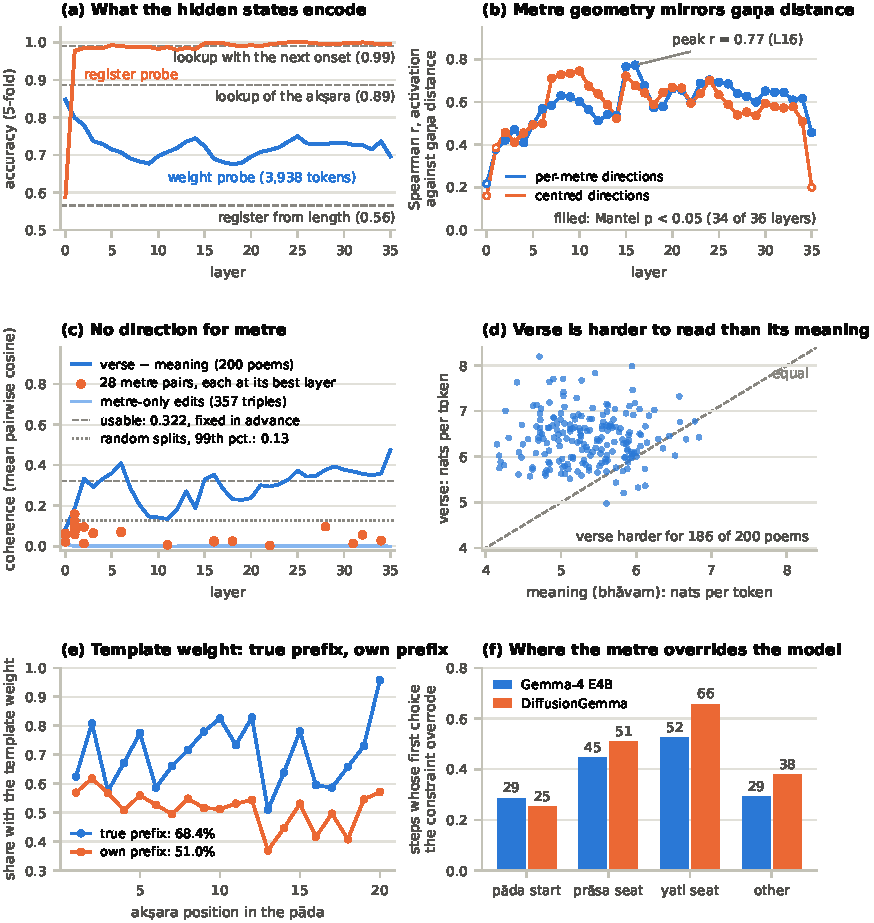
\includegraphics[width=\textwidth]{figures/fig3_experiments.pdf}
\captionof{figure}{The experiments of Table~\ref{tab:diagnostics} as curves. (a)~Accuracy of the weight probe
on the 3,938 tokens whose weight the next akṣara sets \exref{16}, and of the register probe \exref{18}, by
layer, against their baselines. (b)~Spearman r between activation distance and gaṇa distance by layer;
filled points have a one-sided Mantel $p < 0.05$ \exref{19}. (c)~Coherence of the verse $-$ meaning direction
by layer, the best layer of each of the 28 metre pairs \exref{20}, and the metre-only difference of the
tight contrast set \exref{21}. (d)~Mean surprisal per poem of the verse against its meaning, with
\texttt{<bos>} \exref{14}. (e)~The share of akṣaras with the template weight by position in the pāda, with
the true prefix and with the model's own, in the five fixed metres \exref{15}. Panels a--e use
\texttt{gemma-4-E2B-it} \citep{gemma4_2026}. (f)~The share of decoding steps whose first choice the
constraint overrode, by position, over the three strategies, for Gemma-4 E4B \citep{hf_gemma4_e4b} and
DiffusionGemma \citep{hf_diffusiongemma} \exref{22}.}
\label{fig:experiments}\par}


\end{document}
